\documentclass[a4paper,14pt]{extreport}
\usepackage[left=1.5cm,right=1.5cm,
    top=1.5cm,bottom=2cm,bindingoffset=0cm]{geometry}
\usepackage{scrextend}
\usepackage[T1,T2A]{fontenc}
\usepackage[utf8]{inputenc}
\usepackage[english,russian,ukrainian]{babel}
\usepackage{tabularx}
\usepackage{amssymb}
\usepackage{color}
\usepackage{amsmath}
\usepackage{mathrsfs}
\usepackage{listings}
\usepackage{graphicx}
\graphicspath{ {./images/} }
\usepackage{lipsum}
\usepackage{xcolor}
\usepackage{hyperref}
\usepackage{tcolorbox}
\usepackage{tikz}
\usepackage[framemethod=TikZ]{mdframed}
\usepackage{wrapfig,boxedminipage,lipsum}
\mdfdefinestyle{MyFrame}{%
linecolor=blue,outerlinewidth=2pt,roundcorner=20pt,innertopmargin=\baselineskip,innerbottommargin=\baselineskip,innerrightmargin=20pt,innerleftmargin=20pt,backgroundcolor=gray!50!white}
 \usepackage{csvsimple}
 \usepackage{supertabular}
\usepackage{pdflscape}
\usepackage{fancyvrb}
%\usepackage{comment}
\usepackage{array,tabularx}
\usepackage{colortbl}

\usepackage{varwidth}
\tcbuselibrary{skins}
\usepackage{fancybox}


\usepackage{tikz}
\usepackage[framemethod=TikZ]{mdframed}
\usepackage{xcolor}
\usetikzlibrary{calc}
\makeatletter
\newlength{\mylength}
\xdef\CircleFactor{1.1}
\setlength\mylength{\dimexpr\f@size pt}
\newsavebox{\mybox}
\newcommand*\circled[2][draw=blue]{\savebox\mybox{\vbox{\vphantom{WL1/}#1}}\setlength\mylength{\dimexpr\CircleFactor\dimexpr\ht\mybox+\dp\mybox\relax\relax}\tikzset{mystyle/.style={circle,#1,minimum height={\mylength}}}
\tikz[baseline=(char.base)]
\node[mystyle] (char) {#2};}
\makeatother

\definecolor{ggreen}{rgb}{0.4,1,0}
\definecolor{rred}{rgb}{1,0.1,0.1}
\definecolor{amber}{rgb}{1.0, 0.75, 0.0}
\definecolor{babyblue}{rgb}{0.54, 0.81, 0.94}
\definecolor{asparagus}{rgb}{0.53, 0.66, 0.42}
\definecolor{chartreuse}{rgb}{0.5, 1.0, 0.0}
\definecolor{darkorchid}{rgb}{0.6, 0.2, 0.8}

\usepackage{float}
\usepackage{wrapfig}
\usepackage{framed}
%for nice Code{
\lstdefinestyle{customc}{
  belowcaptionskip=1\baselineskip,
  breaklines=true,
  frame=L,
  xleftmargin=\parindent,
  language=C,
  showstringspaces=false,
  basicstyle=\small\ttfamily,
  keywordstyle=\bfseries\color{green!40!black},
  commentstyle=\itshape\color{purple!40!black},
  identifierstyle=\color{blue},
  stringstyle=\color{orange},
}
\lstset{escapechar=@,style=customc}
%}


\begin{document}
\pagecolor{white}

%----------------------------------------1
\newtcbox{\xmybox}[1][red]{on line, arc=7pt,colback=#1!10!white,colframe=#1!50!black, before upper={\rule[3pt] {0pt}{10pt}},boxrule=1pt,boxsep=0pt,left=6pt,right=6pt,top=2pt,bottom=2pt}

\begin{center}\xmybox[amber]{Mnatsakanov Anton} \xmybox[amber]{DP-82} \xmybox[amber]{Variant №5}
\vspace{1cm}

\end{center}


\begin{tcolorbox}[colback=red!5,colframe=red!70!black,title= У чому схожість і різниця акустичних і оптичних фононів?]

First, I want to note that acoustic vibrations of the atomic lattice are electrically inactive, because in this case the electrically neutral (uncharged) center of mass of the unit cell of the crystal is elastically displaced. Accordingly, there is no electric polarization (unless the crystal is polar) due to acoustic vibrations, but optical phonons, on the contrary, are non-acoustic. Also, in a simple atomic crystal with a unit cell consisting of only one atom, there are no optical phonons, but only acoustic (longitudinal and transverse) phonons.
Unlike acoustic vibrations, optical vibrations of ionic crystals are electrically active, i.e. they can be excited by an electric field applied to the crystal. According to the optical oscillations themselves in the crystal are accompanied by fluctuations of electric fields.
 The law of dispersion of acoustic phonons in an ionic crystal is similar to the law of dispersion of LA- and TA-modes in a homeopolar crystal.\\

 As shown in Fig. 1, in addition to acoustic phonons, there are also such
  oscillations at which the displacement phase of neighboring ions differs by almost
  $ dfrac{\pi}{2} $, that is, they move toward each other. The reciprocal displacements of the cation and anion can be both longitudinal and transverse.
    of such elastic oscillations, called optical oscillations, the elastic force is determined by
     by the displacement of the closest neighboring ions and has little dependence on wavelength
      wavelength. Therefore, the frequency of ionic oscillations at a wide variety of wavelengths
       lies in the optical (IR) range.
The corresponding branches of the optical phonon modes LO and TO are shown in the Brillouin zone, Fig. 4.6, г). The dispersion law for optical phonons is quite different from that for
 case of acoustic phonons. When the wave vector k $ \rightarrow 0 $
  (That is, wavelength $ \lambda \rightarrow \infty $), the frequencies of the LO and
   TO do not decrease, as in the case of acoustic phonons, but are directed to finite values $ \omega_{LO} $ i $ \omega_{TO} $.



\tcblower


\end{tcolorbox}

\begin{figure}[h]
\center{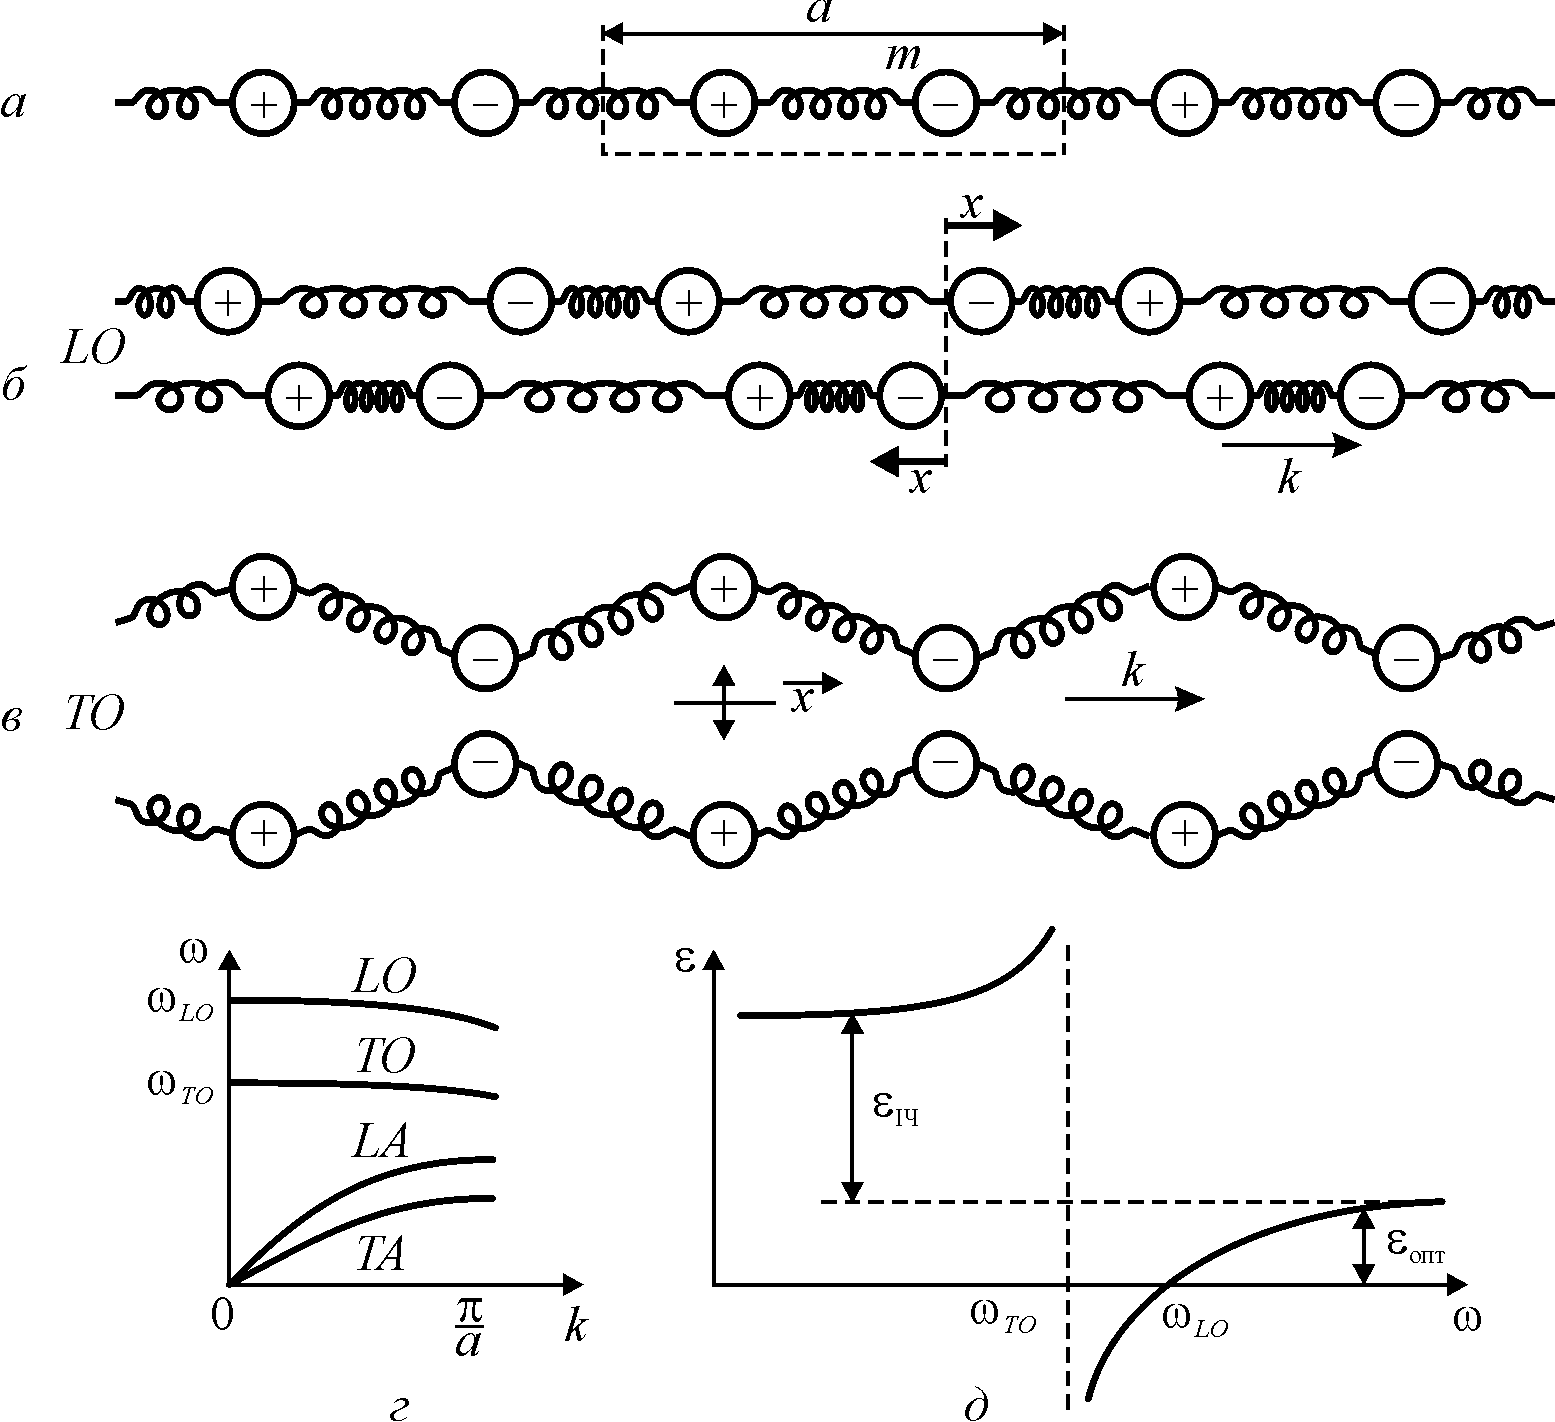
\includegraphics[width=0.7\linewidth]{1.png}}
\caption{Eelastic waves in a one-dimensional ionic crystal: a - chain of elastically coupled ions; b - image of the longitudinal optical wave in the chain; c - image of the transverse optical wave in the chain; d - law of dispersion ("branches") of optical and acoustic waves; e - frequency dispersion of dielectric permittivity.}
\label{ris1}
\end{figure}
\end{document}
